\hsection{Why Python?}%
%
The center of this course is the \python\ programming language.
Our goal is to get familiar with programming, with the programming language \python, and with the tools and ecosystem surrounding it.
This makes sense for several reasons.%
%
\begin{figure}%
\centering%
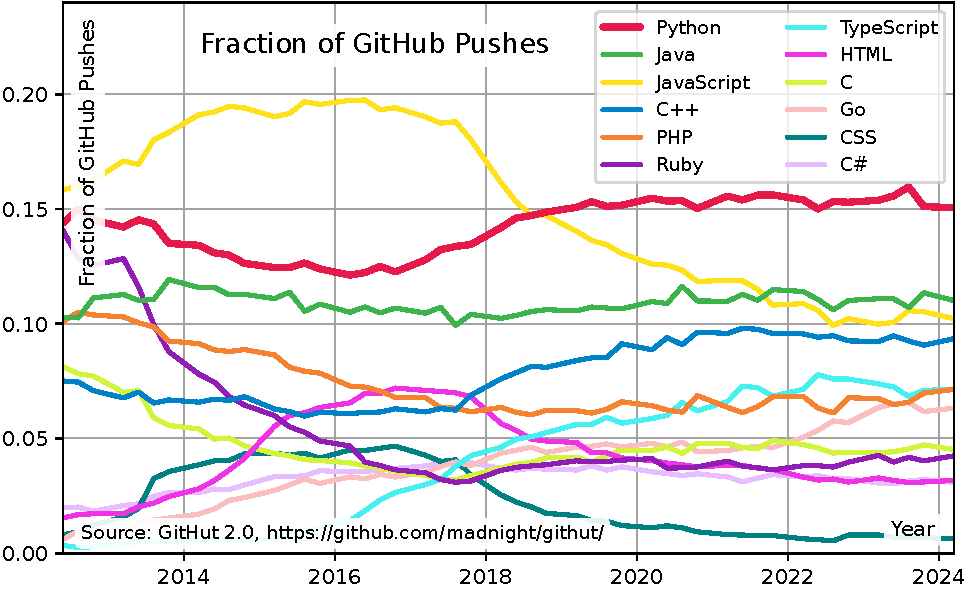
\includegraphics[width=0.75\linewidth]{\currentDir/languagesByGithubPushes}%
\caption{The twelve most popular programming languages chosen based on the \github\ pushes over the years. Source:~\cite{B2023G2GLS}.}%
\label{fig:languagesByGithubPushes}%
\end{figure}%

First, \python\ is one of the most successful and widely used programming languages~\cite{CBST2024LOHPPTDDSAMLA}.
We plot the number of pushes to \github\ over time for the most popular programming and web development languages in \cref{fig:languagesByGithubPushes}.
We find that \python\ became the leading languages at some point in~2018.
In the TIOBE index, which counts the number of hits when searching for a programming language using major search engines, \python\ ranked one in January 2025 and was named the programming language of the year for~2024~\cite{J2025TIFJ2JHPITPLOTY2}.%
%
\cquotation{J2025TIFJ2JHPITPLOTY2}{\python\ is everywhere nowadays, and it is the undisputed default language of choice in many fields.}%
%
If you will do programming in any future employment or research position, chances are that \python\ knowledge will be useful.
According to the 2024 annual Stack Overflow survey~\cite{SESO:DWMMMT2RFSOADS}, \python\ was the second most popular programming language, after \pgls{javascript} and \glslink{HTML}{HTML}/CSS.
In \github's Octoverse Report from October~2024~\cite{GS2024OALPTTLATNOGDS}, \python\ is named the most popular programming language, ranking right before \pgls{javascript}.

Second, \python\ is intensely used~\cite{CBST2024LOHPPTDDSAMLA} in the fields of \pgls{AI}~\cite{RN2022AIAMA}, \pgls{ML}~\cite{SSBD2014UMLFTTA}, and \pgls{DS}~\cite{G2019DSFSFPWP,M2022PFDA} as well as optimization, which are among the most important areas of future technology.
Indeed, the aforementioned Octoverse report~\cite{GS2024OALPTTLATNOGDS} states that the use in soft computing is one of the drivers of \python's popularity.

Third, there exists a very large set of powerful libraries supporting both research and application development in these fields, including \numpy~\cite{HMvdWGVCWTBSKPHvKBHFdRWPGMSRWAGO2020APWN,N2025N,DBvR2024ITN,J2018NPSCADSAWNSAM}, \pandas~\cite{PD2025P,B2012DPWP,L2024PW}, \scikitlearn~\cite{PVGMTGBPWDVPCBPD2011SMLIP,RLM2022MLWPAS}, \scipy~\cite{VGOHRCBPWBvdWBWMMNJKLCPFMVLPCHQHARPvMS2020SFAFSCIP,J2018NPSCADSAWNSAM}, \tensorflow~\cite{ABCCDDDGIIKLMMMSTVWWYZ2016TASFLSML,L2023TDDBTADMLMWT}, \pytorch~\cite{PGMLBCKLGADKYDRTCSFBC2019PAISHPDLL,RLM2022MLWPAS}, \matplotlib~\cite{HDFDM2012MVWP,H2007MA2GE,P2021HOMLPAVWP,J2018NPSCADSAWNSAM}, \simpy~\cite{Z2024DESIEWS}, and \moptipy~\cite{WW2023RSDEWASSAA}\footnote{Yes, I list \moptipy\ here, next to very well-known and widely-used frameworks, because I am its developer.}, just to name a few.
There are also many \python\ packages supporting other areas of computer science, that offer, e.g., connectivity to \pglspl{db}~\cite{VDGE2010P}, or support for web application development~\cite{T2024MFWAAD,A2024FSFAR}.
This means that for many tasks, you can find suitable and efficient \python\ libraries that support your work.

Fourth and finally, \python\ is very easy to learn~\cite{GPBS2006WCTIPIHSUP,VR1999CPFERPASEFTPOT}.
It has a simple and clean syntax and enforces a readable structure of programs.
Programmers do not need to declare datatypes explicitly\footnote{at least during the first steps of learning}.
\python\ has expressive built-in types likes lists, tuples, and dictionaries.
Thus, \python\ was also named the language most popular for those who want to learn how to code in the aforementioned Stack Overflow survey~\cite{SESO:DWMMMT2RFSOADS}.
%
\begin{figure}%
\centering%
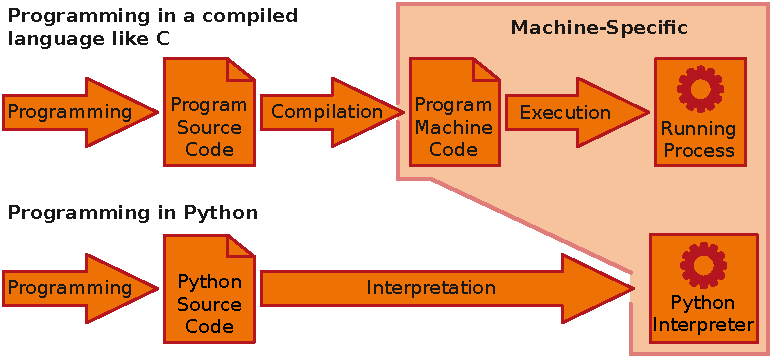
\includegraphics[width=0.7\linewidth]{\currentDir/pythonIsInterpreted.pdf}%
\caption{\python\ code is interpreted, which leads to an easier programming workflow compared to compiled programming languages like \softwareStyle{C}.}%
\label{fig:pythonIsInterpreted}%
\end{figure}%
%
The fact that \python\ is an interpreted language makes it somewhat slower compared to compiled languages like \softwareStyle{C}.
However, this also leads to a much easier workflow when experimenting and programming, as sketched in \cref{fig:pythonIsInterpreted}.
It also is possible to interactively write programs in an interpreter window.
This means that you can execute commands in a \gls{terminal} instead of needing to compile and run programs.
These features, in sum, make \python\ a good choice for learning how to write programs.%
%
\endhsection%
%
